% Lecture 15, Fig. 2: Reid's elastic rebound theory in three stages.
\documentclass[tikz,border=6pt]{standalone}
\usepackage{mathpazo}
\usetikzlibrary{arrows.meta}
\begin{document}
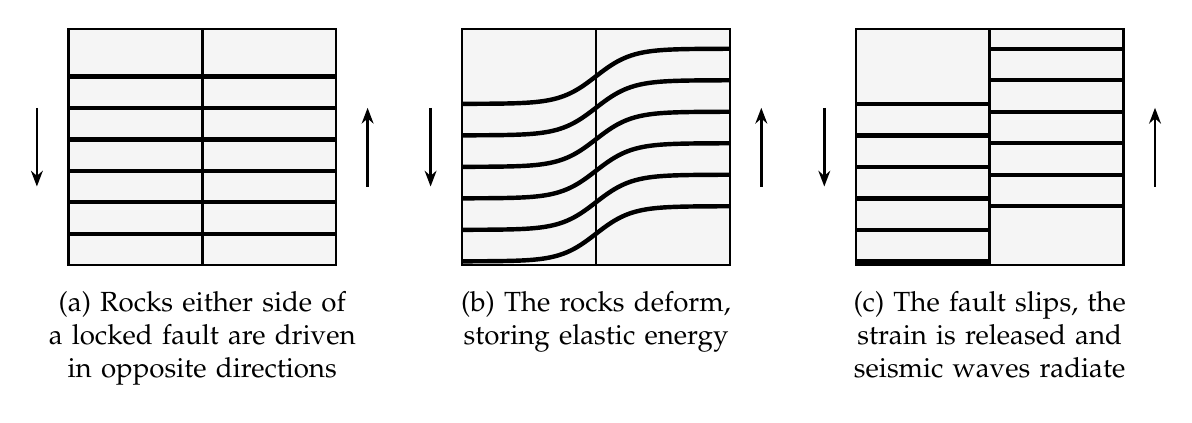
\begin{tikzpicture}[line width=0.8pt]
  \def\D{0.35}   % half the eventual offset
  \foreach \panel/\xoff/\mode/\txt in {a/0/0/{Rocks either side of a locked fault are driven in opposite directions},
                                       b/5/1/{The rocks deform, storing elastic energy},
                                       c/10/2/{The fault slips, the strain is released and seismic waves radiate}} {
    \begin{scope}[shift={(\xoff,0)}]
      \draw[fill=gray!8] (-1.7,-1.5) rectangle (1.7,1.5);
      \foreach \y in {-1.1,-0.7,-0.3,0.1,0.5,0.9} {
        \ifnum\mode=0 \draw[line width=1.6pt] (-1.7,\y) -- (1.7,\y); \fi
        \ifnum\mode=1 \draw[line width=1.6pt,domain=-1.7:1.7,samples=80,smooth] plot (\x,{\y+\D*tanh(2.2*\x)}); \fi
        \ifnum\mode=2 \draw[line width=1.6pt] (-1.7,\y-\D) -- (0,\y-\D); \draw[line width=1.6pt] (0,\y+\D) -- (1.7,\y+\D); \fi
      }
      \draw[line width=1pt] (0,-1.5) -- (0,1.5);          % the fault
      \draw[-{Stealth[length=2mm]},line width=1pt] (-2.1,0.5) -- (-2.1,-0.5);
      \draw[-{Stealth[length=2mm]},line width=1pt] (2.1,-0.5) -- (2.1,0.5);
      \node[anchor=north,text width=4.2cm,align=center,font=\normalsize] at (0,-1.7) {(\panel) \txt};
    \end{scope}
  }
\end{tikzpicture}
\end{document}
